\documentclass[tikz,border=5pt]{standalone}
\usepackage{amsmath}
\usepackage{pgfplots}
\pgfplotsset{compat=1.18}
\usetikzlibrary{arrows.meta}
\definecolor{ink}{HTML}{16324F}
\definecolor{teal}{HTML}{168A88}
\definecolor{gold}{HTML}{D9892B}
\definecolor{redq}{HTML}{B84A4A}
\begin{document}
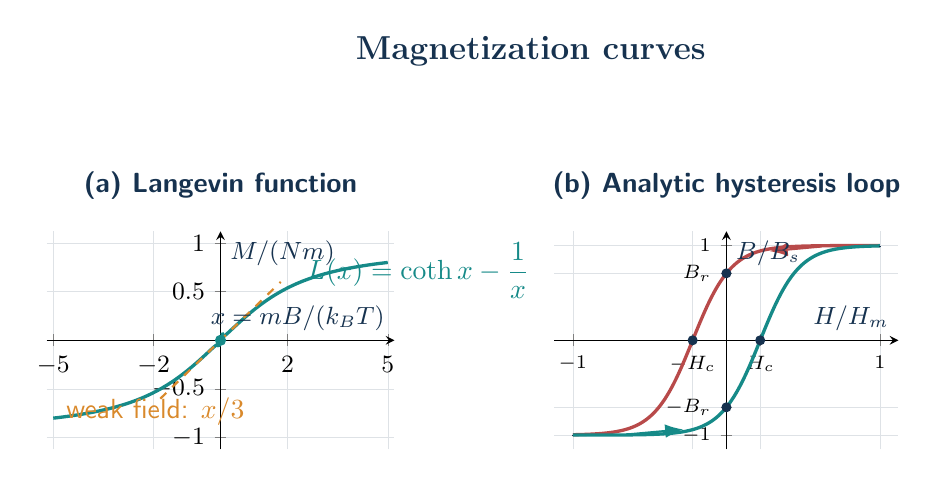
\begin{tikzpicture}[font=\sffamily,>=Latex]
  \node[font=\bfseries\large,ink] at (6.15,5.05) {Magnetization curves};

  \begin{axis}[
    at={(0cm,0cm)},anchor=south west,
    width=6.0cm,height=4.35cm,
    xmin=-5.2,xmax=5.2,ymin=-1.12,ymax=1.12,
    axis lines=middle,
    xlabel={$x=mB/(k_BT)$},ylabel={$M/(Nm)$},
    xtick={-5,-2,0,2,5},ytick={-1,-.5,0,.5,1},
    grid=both,grid style={draw=ink!14,line width=.2pt},
    tick label style={font=\small},
    label style={font=\small,ink},
    title={\bfseries (a) Langevin function},
    title style={ink,yshift=2pt},
    clip=false
  ]
    \addplot[teal,very thick,domain=-5:-.045,samples=220] {1/tanh(x)-1/x};
    \addplot[teal,very thick,domain=.045:5,samples=220] {1/tanh(x)-1/x};
    \addplot[only marks,mark=*,mark size=1.8pt,teal] coordinates {(0,0)};
    \addplot[gold,thick,dashed,domain=-1.8:1.8,samples=80] {x/3};
    \node[teal,anchor=west] at (axis cs:2.3,.72) {$L(x)=\coth x-\dfrac1x$};
    \node[gold,anchor=west] at (axis cs:-4.9,-.73) {weak field: \(x/3\)};
  \end{axis}

  \begin{axis}[
    at={(6.45cm,0cm)},anchor=south west,
    width=5.95cm,height=4.35cm,
    xmin=-1.12,xmax=1.12,ymin=-1.15,ymax=1.15,
    axis lines=middle,
    xlabel={$H/H_m$},ylabel={$B/B_s$},
    xtick={-1,-.22,0,.22,1},
    xticklabels={$-1$,$-H_c$,$0$,$H_c$,$1$},
    ytick={-1,-.707,0,.707,1},
    yticklabels={$-1$,$-B_r$,$0$,$B_r$,$1$},
    grid=both,grid style={draw=ink!14,line width=.2pt},
    tick label style={font=\scriptsize},
    label style={font=\small,ink},
    title={\bfseries (b) Analytic hysteresis loop},
    title style={ink,yshift=2pt},
    clip=false
  ]
    \addplot[redq,very thick,domain=-1:1,samples=241]
      {tanh(4*(x+.22))/tanh(4*1.22)};
    \addplot[teal,very thick,domain=-1:1,samples=241]
      {tanh(4*(x-.22))/tanh(4*1.22)};
    \addplot[ink,densely dotted] coordinates {(-1,{tanh(4*(-1-.22))/tanh(4*1.22)}) (-1,{tanh(4*(-1+.22))/tanh(4*1.22)})};
    \addplot[ink,densely dotted] coordinates {(1,{tanh(4*(1-.22))/tanh(4*1.22)}) (1,{tanh(4*(1+.22))/tanh(4*1.22)})};
    \addplot[only marks,mark=*,mark size=1.6pt,ink] coordinates {(-.22,0) (.22,0) (0,.7067) (0,-.7067)};
    \draw[->,redq,thick] (axis cs:.62,.99)--(axis cs:.28,.94);
    \draw[->,teal,thick] (axis cs:-.62,-.99)--(axis cs:-.28,-.94);
  \end{axis}
\end{tikzpicture}
\end{document}
